\chapter{INTERFACE DEVELOPED FOR THE BLENDER GAME ENGIME}\label{chap5}

% introduction
%\section{Introduction}

% video game history
Video games have been around since the 1950s\cite{historyVideoGames}. They became available in the market by the 1970s, at that time they were very popular. Currently, games are the attraction of many people. There are all kinds of video games available now. There are consoles games, portable consoles games, computer games, cell phones games, etc. Video games are everywhere. 

% our aim
Our aim is to develop tools that would help to create games, but not any kind of games, we focus on \textit{educational games}. Educational games are those that not only the player enjoys while he/she is playing but also the player learns through it. 

%The\textit{Blender Game Engine} was chosen as the software to enhance in this project. The work presented in this thesis is done for the \textit{Blender Game Engine} which lacks Particle Systems.

% layout of the chapter
This chapter starts with a brief discussion of what is \textit{Blender}, followed by a description of its \textit{Game Engine}. Then, the Boids particle system outside the Blender Game Engine will be presented, and finally the modifier developed for the use of the RTPS library is described.

% blender background info
\section{Blender}\label{blenderSec}
\textit{Blender}\cite{blenderWeb} is a free modeling/simulation software that has been out since 1993, at the beginning it was mostly used to create 2D and 3D content. Currently, it has been extended and it can also do modeling, texturing, animation, particle simulation, rendering, game creation, etc.

When searching for the right software to use, the following properties of Blender made it the top software in the list. Blender has a free built-in game engine, it can be extended (Open Source project), it is cross-platform i.e. it can be used in either Windows, MacOSX and Linux, and it can support simulations with real physics. Blender also has a big support from the gaming industry, and there is a large community helping with tutorials and documentation.

The Blender release used in this thesis was 2.57.

% game engine
\section{Game Engines}

% what is a game engine?
A game engine is a software or part of a software that simulates partial reality\cite{bookGameKit2}. Game engines let you interact with 3D world in real-time. Also, they let you control objects that interact with other objects in the world. 

Game engines has several tasks:
\begin{enumerate}
\item{render the 3D world and the objects on it}
\item{re-render the scenes when something in the world changes}
\item{game logic, decide what to do when the game is being played}
\item{simulate the physics of the game i.e. gravity}
\item{collision detection and reaction}
\end{enumerate}

Game engines try to simulate the scenes as quickly as possible, so the game has a smooth fluency. Game engines are much more complicated than this, these are just a few of the most important jobs that characterize them.

% blender game engine
As mentioned in Section~\ref{blenderSec} Blender has a \textit{Game Engine} built-in. The Blender Game Engine is a very powerful tool, it allows simple games to be created without  the need for explicit programming. With its GUI you are able to create simple games just by clicking and dragging. After creating the 3D objects and 3D world you can use the simple logic editor to bring the scene to life. The logic editor interface is shown in Figure~\ref{logic}.

\begin{figure}[htbp]
\begin{center}$
\begin{array}{c}
%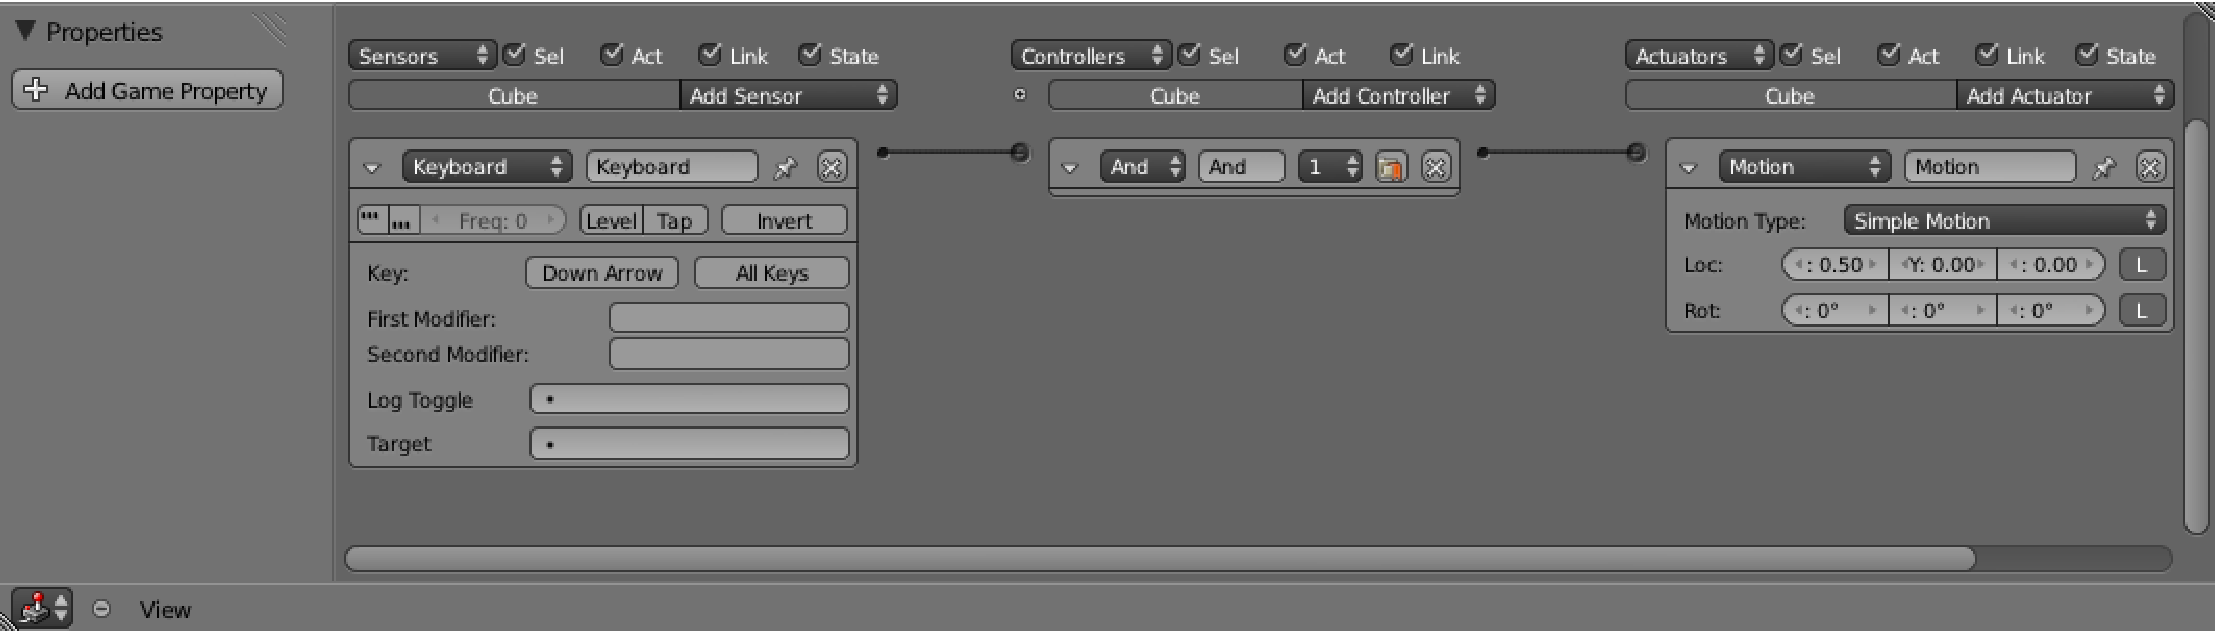
\includegraphics[scale=0.4]{figures/logic.pdf}
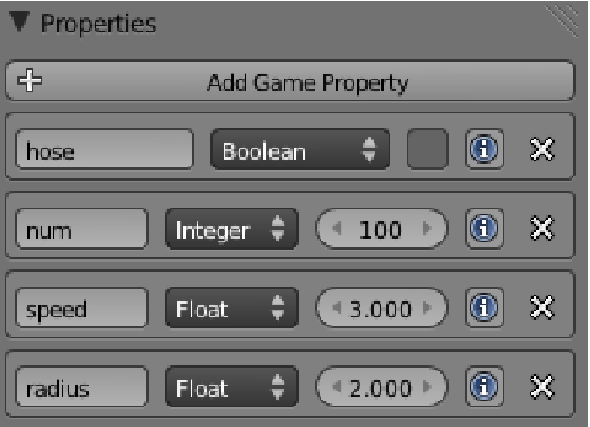
\includegraphics[scale=0.5]{figures/demo1_logic_properties.pdf} \\
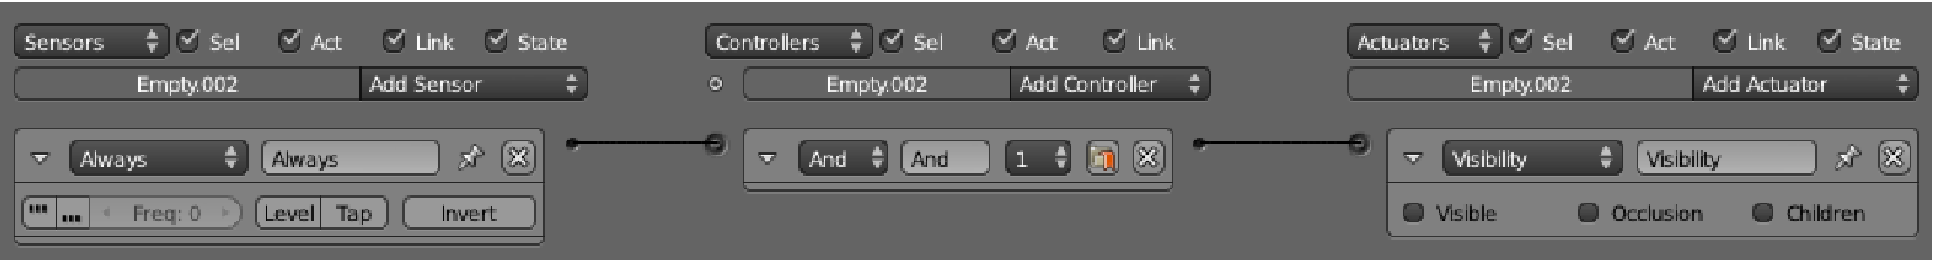
\includegraphics[scale=0.45]{figures/demo1_logic_bricks.pdf}
\end{array}$
\end{center}
\caption{The Blender Game Engine Logic Editor interface: consists of the Properties and the Logic Bricks areas}
\label{logic}
\end{figure}

The logic editor interface consists of two parts: \textit{Properties} and \textit{Logic Bricks}. Properties are used to give more specific actions to the objects, these properties can be called using the variables' names. The name of the variables has to match with the implementation in the source code. The second part is the logic bricks. The logic bricks are divided into \textit{sensors}, \textit{controllers}, and \textit{actuators}. Each of these has different subtypes to chose from.

Sensors are used to detect the input from the user e.g. sensors can be from the keyboard, mouse, joysticks, etc. Controllers link the Sensors with the Actuators, using Controllers you can decide what action to take after the input has been received. The Actuators make the actual action within the game. As an example the object might move, rotate, create, destroy, change in shape, etc.

To create logic for an object in the world you just have to add as many logic bricks you need, and do not forget to connect them by dragging the connector from the sensor to the controller and from the controller to the actuator. The example move showed in Figure~\ref{logic} shows the forward movement of a cube using the down arrow.

This is the simplest way to create life within the world. For more complex behavior you can extend the capabilities by using the Python scripting interface.

% particle system outside the blender game engine
\section{Boids Particle System outside the Blender Game Engine}
Although Blender has extensive particle-based tools, including hair styling, these are absent from the Game Engine. A submodule of the particle system is a rather sophisticated Boid system. This section presents a demo that shows how this Boid system works.

First you need to create a particle emitter, it can be a cube, a plane, or any other object. Then, make that object the particle system. Figure~\ref{boidsCreatePS} shows the panel used to add the particle system. The amount of particles is set to 50, using the starting and ending time as 1 would make the simulation to be calculated at each time step, there is no repetition (oscillation) in the behavior of the boids. The lifetime is set to a big number to keep our boids alive for long time. Using these settings would be as much as can be done to run real-time-like simulation using the Boids system of Blender.

% figure: create PS
\begin{figure}[htbp]
\begin{center}
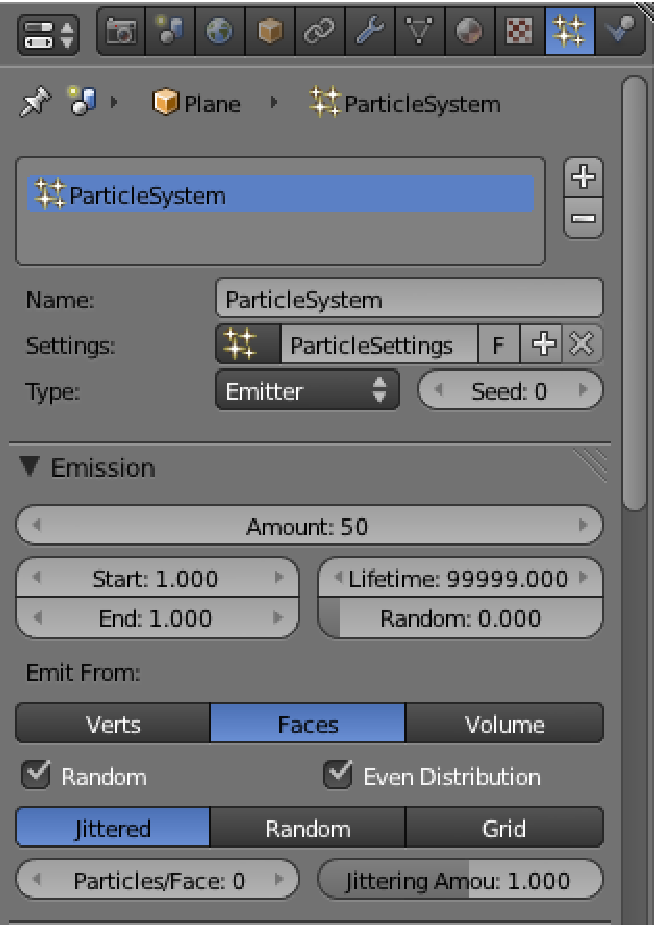
\includegraphics[scale= 0.65]{figures/boidsCreatePS.pdf} 
\caption{Blender Particle Systems Add and Emission panels: add a particle system and set the number of particles in that particle system}
\label{boidsCreatePS}
\end{center}
\end{figure}

After the system is created, the physics of the system can be edited, see Figure~\ref{boidsPhysics}. First, click on \textit{Boids}, and all the settings of the Boids system will show up. Settings can be changed dynamically while the animation is running.

% figure: boids physics
\begin{figure}[htbp]
\begin{center}
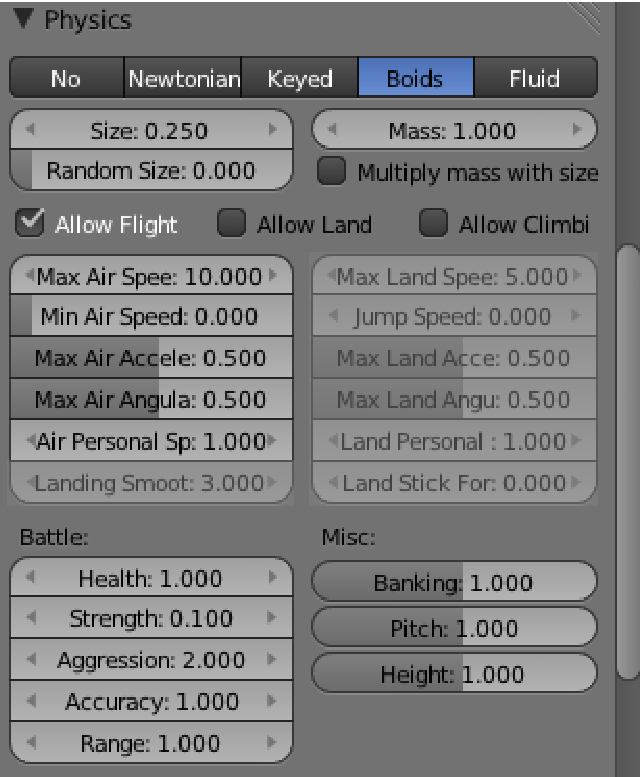
\includegraphics[scale = 0.65]{figures/boidsPhysics.pdf} 
\caption{Blender Particle Systems Physics panel for Boids: set the physical properties of the Boids particle system}
\label{boidsPhysics}
\end{center}
\end{figure}

In Blender Boids system the boids have their own brain, therefore more specific settings can be assigned depending on the application. Figure~\ref{boidsBrain} shows the panel for the Boids Brain. Next, is a list of the rules available in Blender\footnote{Description of rules is listed as it is in the Blender source code.}.

%Blender boid's rules
\begin{enumerate}
\item{Goal: go to the goal assigned object or loudest assigned signal source}
\item{Avoid: get away from assigned object or loudest assigned signal source}
\item{Avoid Collision: maneuver to avoid collisions with other boids and deflector object in near future}
\item{Separate: keep from going through other boids}
\item{Flock: move to center of neighbors and match their velocity}
\item{Follow Leader: follow a boid or assigned object}
\item{Average Speed: maintain speed. flight level or wander}
\item{Fight: go to closest enemy and attack when in range}
\end{enumerate}

When clicking in a rule, if that rule needs some extra parameters, the respective input areas will show up. As seen in Figure~\ref{boidsBrain}, after clicking the rule Goal the option to set which object is the target shows. An empty object created by us was set as the target. 

There are three methods available in Blender to evaluate the rules. Those methods are fuzzy logic with a fuzziness level, averaging all rules, and weighting the rules randomly. Each of these evaluation methods leads to completely different results. The default type of rules evaluation method is Fuzzy.

The render panel, also seen in Figure~\ref{boidsBrain} shows the options for rendering the flock. Here we changed the rendering type to object and set a monkey object to be the object to be render as a boid.

% figure: boid brain
\begin{figure}[htbp]
\begin{center}
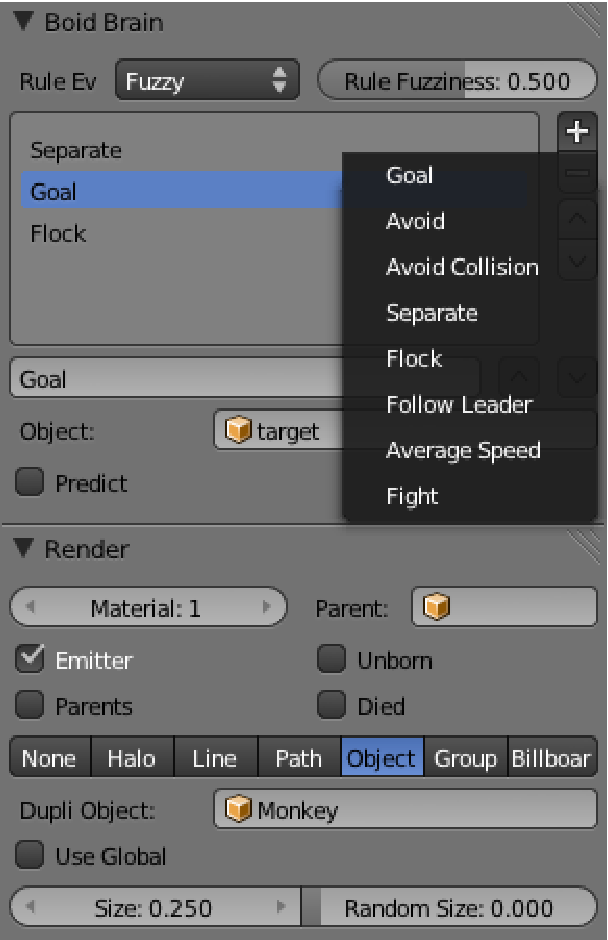
\includegraphics[scale = 0.65]{figures/boidsBrain.pdf}
\caption{Blender Particle Systems Boid Brain and Render panels: set the rules that the boids are going to follow, and set the render type}
\label{boidsBrain}
\end{center}
\end{figure}

Figure~\ref{boidsAction} shows two screenshots of an animation in which the boids are approaching an empty object as the target. This animation was running using the settings presented in the previous Figures.

% figure: boids in action
\begin{figure}[htbp]
\begin{center}$
\begin{array}{cc}
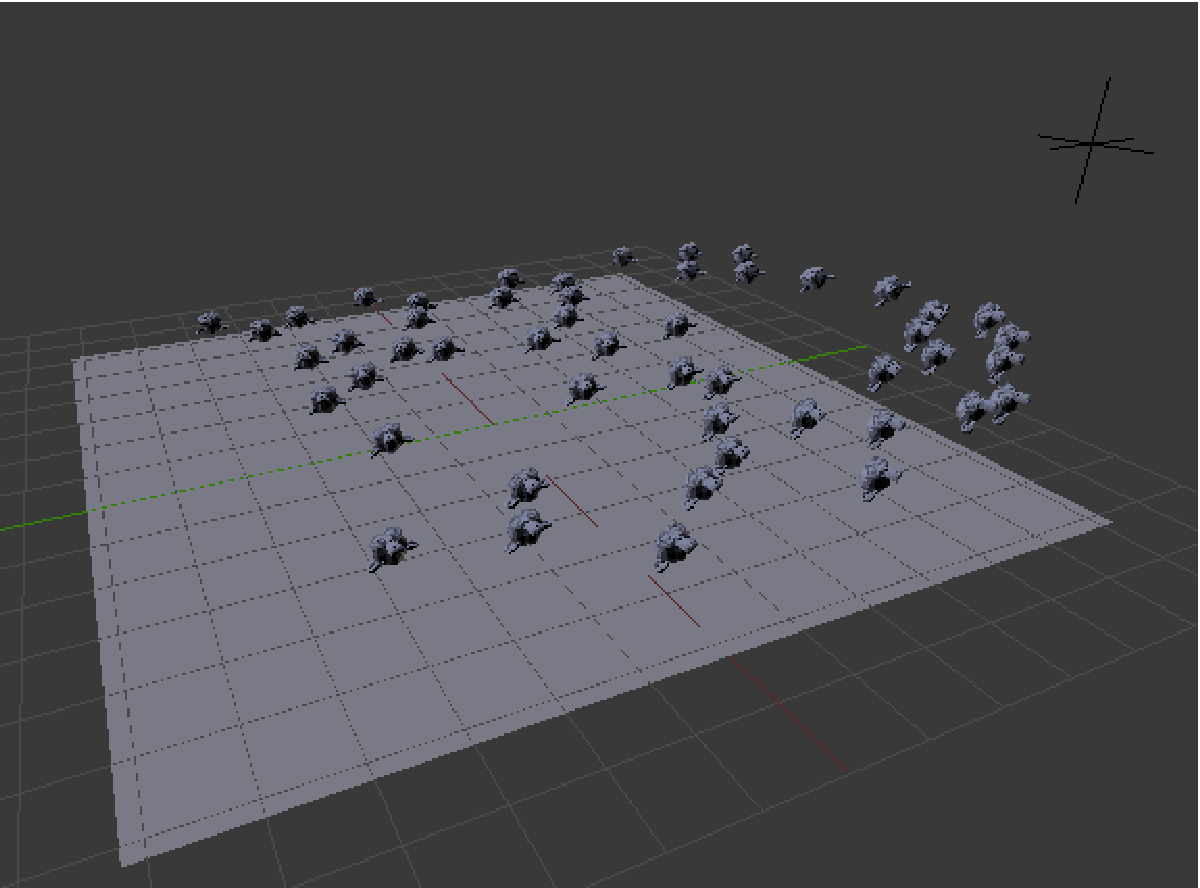
\includegraphics[scale= 0.35]{figures/boids1.pdf} &
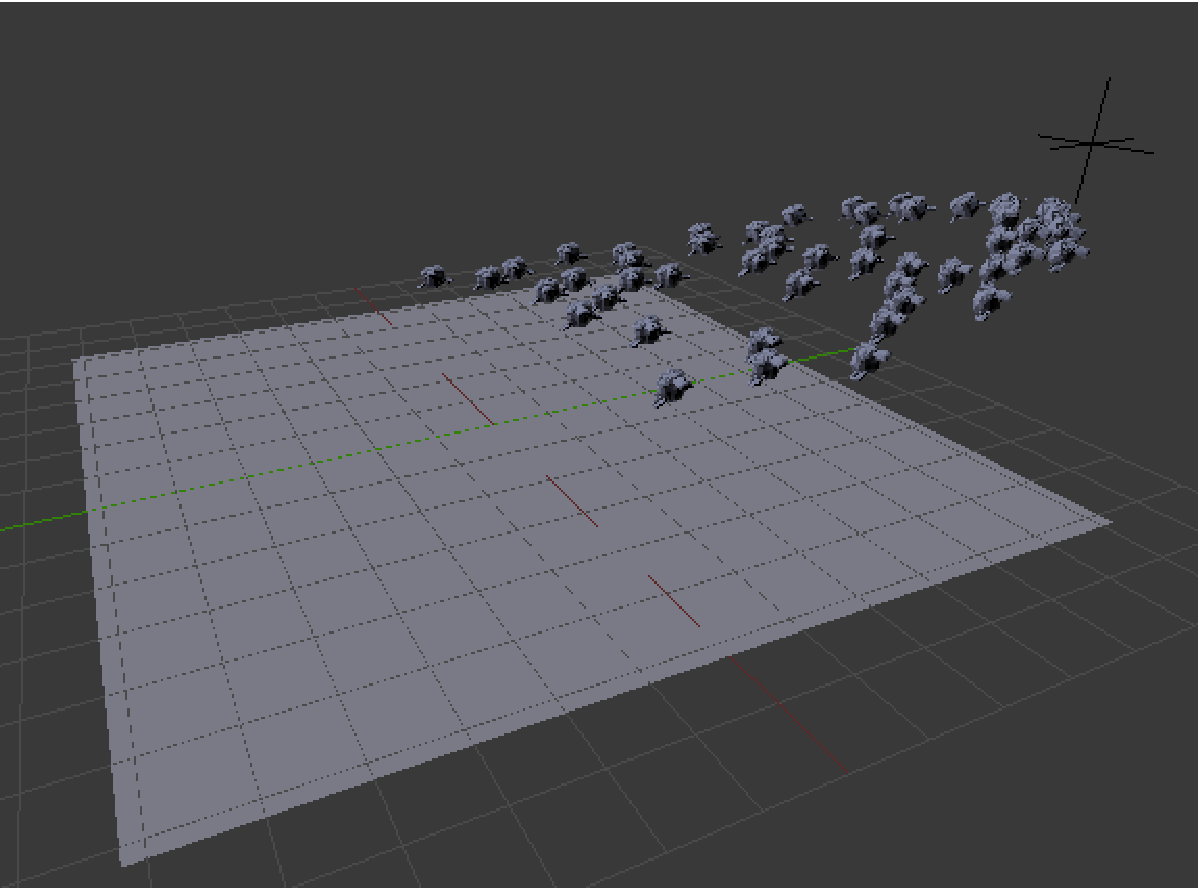
\includegraphics[scale= 0.35]{figures/boids2.pdf}
\end{array}$
\end{center}
\caption{Screenshots of the boids approaching an empty object as the target}
\label{boidsAction}
\end{figure}

% RTPS modifier
\section{RTPS Modifier}\label{modifiersection}
This section presents the interface developed to link the Blender Game Engine with our FLOCK system defined in the RTPS library. This interface is a custom modifier. Modifiers are used to edit the object by assigning certain properties to it. For example in our case, first we create the domain using a Blender cube and then assign the RTPS modifier to it. 

For a step by step description on how this modifier was created see Ian Johnson post at http://enja.org/2010/05/24/blender-creating-a-custom-modifier/.  The functionality of the Boids system was added to the original RTPS modifier which was created to support only SPH systems. 

% code modifications
\subsection{Game Engine Source Code Modifications}
To create the custom modifier a few files have to be modified. These modifications are divided into three categories: Functionality of the Game Engine, Functionality of the UI Modifier, and  Creation of the UI Modifier.

The main changes made to the Blender source code are summarized in Tables~\ref{geTable},~\ref{funcTable},~\ref{uiTable}.

% tables summarizing the changes made to the source code

% GE table
\begin{table}[htdp]
\caption{Modifications made for the functionality of the Game Engine}
\begin{center}
\begin{tabular}{|p{6cm}|p{6cm}|}
\hline 
\textbf{File} & \textbf{Summary of the Modifications} \\\hline 
BL\_BlenderDataConversion.cpp & Checks if the RTPS modifier is been used. \\\hline 
BL\_ModifierDeformer.cpp & Implementation of all the functionality of RTPS inside Blender. The RTPS object is created and update it every frame. \\\hline 
RAS\_ListRasterizer.cpp & Calls the \texttt{render()} method. \\
\hline 
\end{tabular} 
\end{center}
\label{geTable}
\end{table}

% Functionality table
\begin{table}[htdp]
\caption{Modifications made for the functionality of the UI modifier}
\begin{center}
\begin{tabular}{|p{6cm}|p{6cm}|}
\hline 
\textbf{File} & \textbf{Summary of the Modifications} \\\hline 
DNA\_modifier\_types.h & Defines the \texttt{struct} of the RTPS modifier. \\\hline 
rna\_modifer.c & Defines the properties of the items in the UI. \\\hline 
MOD\_rtps.c & This file was created and defines the default values of the parameters in the UI. \\
\hline 
\end{tabular}
\end{center}
\label{funcTable}
\end{table}

% UI table
\begin{table}[htdp]
\caption{Modifications made for the creation of the UI modifier}
\begin{center}
\begin{tabular}{|p{6cm}|p{6cm}|}
\hline 
\textbf{File} & \textbf{Summary of the Modifications} \\\hline 
properties\_data\_modifier.py & Creates the UI modifier using the properties defined in \texttt{rna\_modifier.c}. \\
\hline 
\end{tabular}
\end{center}
\label{uiTable}
\end{table}

% UI description
\subsection{Development of the UI}
Our RTPS modifier as the Blender interface is implemented using \textit{Python}. As described in table~\ref{uiTable} the only file modified for the development of the UI was \texttt{properties\_data\_modifier.py}. The RTPS modifier is shown in Figure~\ref{ui}.

% figure: RTPS modifier
\begin{figure}[htbp]
\begin{center}
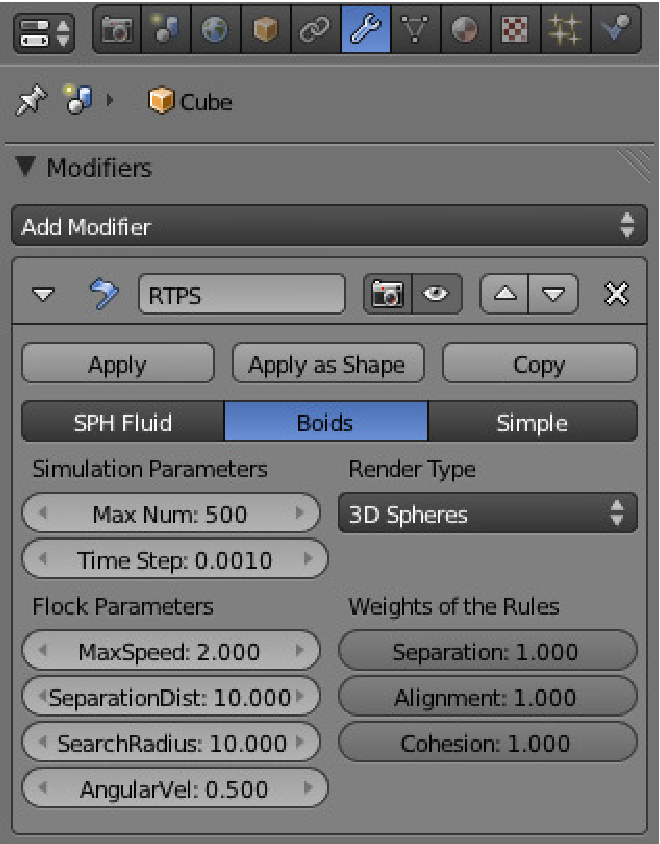
\includegraphics[scale=0.8]{figures/modifier.pdf}
\caption{Boids system of the RTPS modifier: it includes the simulation parameters, the render types, the flock specific parameters, and the weights for each of the rules; here showing the default values}
\label{ui}
\end{center}
\end{figure}

The RTPS modifier is used to initialize one of the three particle systems available in the RTPS library. The Boids systems has the options to set the simulation parameters which are the maximum number of particles and the time step used for integration.  Next to the simulation parameters is the Render types area which includes the options to render the boids as Points, Sprites, Screen Space, and 3D Spheres. The color used to render the particles is gotten from the Materials section of Blender.

The Flock Parameters area you can specify the maximum speed of the boids, the minimum separation distance that is going to be kept by the boids and the searching radius for the neighbor search. The last area of the Boids interface is the Weights of the Rules area, here you are able to specify how much do you want each of your rules to be weighted when they are evaluated. These weights are the constant values of Equation~\ref{combine}.

\textit{How does the RTPS modifier works internally?} The modifier is applied to the object when the game engine starts. In the RTPS modifier \textit{Apply} means that the RTPS object is created and initialized using the current parameters in the modifier. After, the RTPS object is created it can be updated. The object is updated at every frame.    

\textit{How to emit particles into the system?} They are two emitters available in the RTPS modifer: \textit{Blob} and \textit{Hose}. You can use these emitters by setting the respective properties. See the description of the properties defined for the RTPS objects in Table~\ref{properties}. If using \textit{Blob}, the only needed property is \texttt{num}, and for \textit{Hose} emitter you would need to use \texttt{num}, \texttt{speed}, and \texttt{radius}. The direction in which the particles are emitted when using the \textit{Hose} is determined by the \textit{y-axis} of the emitter object. 

% properties table
\begin{table}[htdp]
\caption{Properties available in the RTPS modifer}
\begin{center}
\begin{tabular}{|p{3cm}|p{9cm}|}
\hline 
\textbf{Property} & \textbf{Type and Description} \\\hline 
\texttt{num} 	& \texttt{integer}: if num $>$ 0, num particles are going to be emitted every frame and num is set to 0	\\\hline 
\texttt{hose}	& \texttt{boolean}: used to active the hose	\\\hline
\texttt{speed}	& \texttt{float}: initial velocity of the particles that are going to be emitted from the hose	\\\hline
\texttt{radius}	& \texttt{float}: width of the hose	\\ %\hline
%\texttt{index}	& \texttt{integer}: used when more than hose is been used in the game	\\\hline
%\texttt{refill}	& \texttt{integer}: 	refill the hose \\\hline
%\texttt{collider}	& \texttt{boolean}: used to active collisions detections in the SPH system	\\
\hline 
\end{tabular}
\end{center}
\label{properties}
\end{table}

